\chapter{Multi-Agent Stochastic Target Localization}
\placeholder{}
This chapter outlines the approach taken to solve the research question stated in the introduction chapter. The context for this problem is derived from the ROCSAFE project \cite{rocsafeNUIG}. \note{Not sure how best to present the problem and how to provide the necessary content to naturally leads to the approaches discussed here. Fill this out further once research questions have been finalized/refined}

%%%%%%%%%%%%%%%%%%%%%%%%%% Bayesian Filtering Sections %%%%%%%%%%%%%%%%%%%%%%%%%%
\section{Bayesian Filtering for State Estimation}
\note{Rename this to stochastic search algorithms or something else}

\subsection{Hidden Markov Models}
\nomenclature[]{HMM}{Hidden Markov Model}
\placeholder{}
\note{Could discuss:
\\Background
\begin{itemize}
    \item What HMMs are
    \item why they're useful in AI
    \item the different commonly used HMMs. 
\end{itemize}
\\ Use in my research:
\begin{itemize}
    \item How the problem can naturally be described by a HMM
    \item Lead into discussion of how DBN is a more natural way to describe the problem and how it leads to efficient factorization of densities for state estimation
\end{itemize}
}
Hidden Markov Models appear frequently in AI literature as they provide an abstract framework to deal with stochastic processes, which themselves are pervasive in their use as a tool to model real-world phenomena. This chapter will outline what HMMs are and their use in literature describing target localization algorithms. A general overview of HMMs can be found in \cite{Murphy1994DynamicLearning}\cite{Ghahramani2001ANNETWORKS}.

\subsubsection{Markov Processes}
It is instructive to understand what is meant by a stochastic process for some of the concepts mentioned in this thesis. The high-level details will be discussed here and the reader can refer to a text on probability theory for a fuller explanation, for example \cite{papoulis02}. A random process can be described as a family of random variables indexed by a set $\tau$: $\{X_t\}_{t\in\tau}$. Commonly in AI, stochastic processes model the evolution of a random system through \textit{discrete} time steps: $\tau$=$\mathbb N$. Common phenomena modelled by stochastic processes include the growth of a bacterial population and the movement of a gas molecule.\par

A first-order discrete-time Markov process is a stochastic process that describes a system which is in a given state at each time step, with the state changing randomly between steps. The steps are elements of the natural numbers and the random process is a mapping from the natural numbers to states. First-order Markov processes have the additional property that the probability distribution of the n$_{th}$ random variable in the process is conditionally independent of all previous probability distributions in the sequence but the $n-1_{st}$: $P(X_t = x_t | X_{t-1} = x_{t-1}, X_{t-2} = x_{t-2}, ... , X_{1} = x_{1}) = P(X_t = x_t | X_{t-1} = x_{t-1})$. This is often referred to as the Markov Property or the memoryless property of Markov processes. In order to describe a Markov process, it is therefore necessary to describe what is known as the transition function between each pair of timesteps: $P(X_t = x_t | X_{t-1} = x_{t-1})$. A common assumption is that the rules that govern state transitions are time invariant, meaning that they can be specified generally for any given pair of timesteps. This assumption will be made for the subsequent discussion. If $X_t$ is a discrete random variable defined over $S$ states, the transition function can be described by a stochastic matrix T, where T$_{i,j}$ = $P(X_t = j | X_{t-1} = i)$: 

\begin{center}
{$\displaystyle \left({\begin{matrix}T_{1,1}&T_{1,2}&\dots &T_{1,j}&\dots &T_{1,S}\\T_{2,1}&T_{2,2}&\dots &T_{2,j}&\dots &T_{2,S}\\\vdots &\vdots &\ddots &\vdots &\ddots &\vdots \\T_{i,1}&T_{i,2}&\dots &T_{i,j}&\dots &T_{i,S}\\\vdots &\vdots &\ddots &\vdots &\ddots &\vdots \\T_{S,1}&T_{S,2}&\dots &T_{S,j}&\dots &T_{S,S}\\\end{matrix}}\right)$}
\end{center}
\par

Some obvious results are worth pointing out; as for any stochastic matrix, by the axioms of probability theory, the sum of conditional probabilities across {$\displaystyle \sum _{j=1}^{S}T_{i,j}=1$} and the transition probabilities over k timesteps can be described by the $k_{th}$ power of the transition matrix: ${(T^k)}_{i,j}$ = $P(X_{t+k} = j | X_{t} = i)$. Markov processes are often described by graphical models, for example Figure \ref{fig:markov-processes}.
\begin{figure}[b]
    \centering
    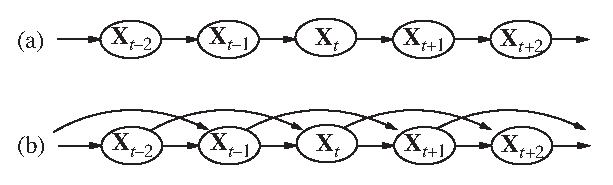
\includegraphics{Chapters/MultiAgentProbabilisticSearch/BayesianFiltering/Figs/markov-processes.eps}
    \caption{First (a) and second (b) order Markov processes \cite{AIAMA}}
    \label{fig:markov-processes}
\end{figure}
It also is possible to calculate the probability of the process experiencing a sequence of states from timesteps 1 as far as t, using the chain rule of probability and the Markov property:
$P(X_{1:t}) = P(X_1, X_2, ..., X_t) = P(X_1)\times P(X_2 | X_1)\times P(X_3 | X_2, X_1) \times P(X_t | X_{t-1}, X_{t-2}, ... , X_1) = P(X_1) \times \prod_{i=2}^{t}{P(X_i | x_{i-1})}$. Marginalization over variables in this sequence allows the calculation of many useful quantities.
\par

\subsubsection{HMM Description}
Hidden Markov Models (HMMs) are models that build on the Markov Process model, which describe the evolution of a random system in the language of probability theory. HMMs assume that the system being modeled can be described by a Markov process, but that the states of this process are unobservable. This means that it isn't possible to determine the state of the system exactly at any given point in time. However, it is possible to make an observation of a random variable that is related to the hidden state which yields information about the hidden state. This is visualised in Figure \ref{fig:hmm}
\begin{figure}[]
    \centering
    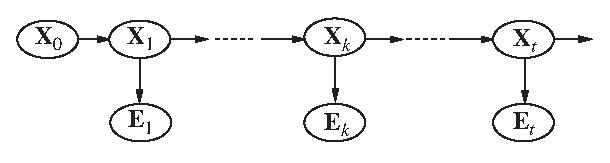
\includegraphics{Chapters/MultiAgentProbabilisticSearch/BayesianFiltering/Figs/smoothing-dbn.eps}
    \caption{A visualisation of a HMM \cite{AIAMA}}
    \label{fig:hmm}
\end{figure}
, where the Markov Process is shown by the variables $X_i$ and the observation variables are shown by variables $E_i$. A HMM can be specified by a triple, $\lambda$ = $(T, O, \pi)$, where $T$ is the stochastic transition matrix, $\pi$ is the initial distribution $P(X_1)$ and O describes the conditional probability of an observation given that the system is in a certain state: $O(E_i, X_i) = P(E_{i} | X_{i})$. Taken together, it is then possible to specify the joint distribution of the hidden state variables and the evidence variables, analogous to the Markov Process: 
$
P(X_{1:t}, E_{1:t}) = P(X_1, X_2, ..., X_t, E_1, E_2, ..., E_t) = P(X_1) \times P(E_1 | X_1) \times
\prod_{i=2}^{t}{(P(X_i | x_{i-1}) \times P(E_t | X_t))}.
$Given representation, it is then possible to answer questions such as:
\begin{itemize}
    \item Given the HMM, $\lambda$, determine the probability of occurrence of a particular observation sequence, $P(E_{1:t} | \lambda)$
    \item Given a sequence of observations $(E_1, E_2, ..., E_n)$, what is the most likely sequence of hidden states that led to these observations? i.e. find \[\argmax_{X_{1:t}} P(X_{1:t} | E_{1:t})\].
    \item Determine the parameters of $T$ and $O$, given a training set of observations, i.e. find the solution to \[\argmax_{\lambda} P(E_{1:t} | \lambda)\].
    \item Filtering: What is the current distribution of the hidden state given all previous evidence ('belief state') of the agent at time t: $P(X_t | E_{1:t})$?
    \item Prediction: What is the distribution of the hidden state in the future, given all evidence to date: $P(X_{t+k} | E_{1:t})$, for some k$>$0?
    \item Smoothing: What is the distribution of a past state given all observations up to the current point in time: $P(X_k | E_{1:t})$, for some 0 $\leq$ k $<$ t?
\end{itemize}
\par

%Might include a subsection on a taxonomy of commonly used HMMs.

\subsubsection{Summary}
In summary, HMMs can be used to abstractly describe the evolution of a stochastic system. They have been used to achieve state of the art performance in problems such as speech recognition \cite{ChiuSTATE-OF-THE-ARTMODELS} and ... . An comprehensive overview of extensions to the vanilla HMM can be found at \cite{Murphy1994DynamicLearning}.
\label{Chapter:HMM}

\subsection{Dynamic Bayesian Networks}
\nomenclature[]{DBN}{Dynamic Bayesian Network}
\nomenclature[]{BN}{Bayesian Network}
\nomenclature[]{CPD}{Conditional Probability Distribution}
\nomenclature[]{2TDBN}{2 Time Slice Dynamic Bayesian Network}

\placeholder{}
Dynamic Bayesian Networks are a generalization of HMMs and are used to model time series, without being limited to the assumptions of HMMs. The key difference between DBNs and HMMs is that DBNs are not limited in how they decompose the state of a complex stochastic system into the variables that represent its constituent distributions \cite{AIAMA}. Technically, every DBN can be represented as a HMM and visa versa, however, the number of parameters that need to be detemined to represent DBNs can be significantly less that that of HMMs. This is a manifestation of how specifying a full joint discrete distribution can require an exponential number of probabilities, whereas specifying the same joint distribution as factored conditional distributions may require far fewer.

\subsubsection{A Note on Bayesian Networks}
A Bayesian Network (BN) is a graphical way to represent a particular factorization of a joint distribution. For a detailed explanation, the reader is referred to \cite{KollerPGM}. To fully explain a complex system, it is often natural to model it as the joint distribution of a number of random variables. This is in general intractable \cite{KollerPGM}. In order to circumvent this, independence properties in the distribution can be exploited to provide a much more compact representation of the distribution. BNs exploit the fact that independence is a strong notion that doesn't often occur in the real-world; however conditional independence is a weaker property that is far more prevalent, which still leads to the desired compact representation. BNs are described by a directed acyclic graph (DAG), $G$. The nodes in the graph correspond to the random variables whose joint distribution is of interest, and the arcs represent conditional independences. Specifically, if one Burglary points to Alarm as in figure \ref{BayesianNetwork}, it is implied that the distribution of Alarm is conditionally independent on all other nodes in the network given Burglary. This means that only local conditional probability distribution must be provided in order to specify the full joint distribution.

\begin{figure}
%example bayesian network figure
\begin{tikzpicture}[
  node distance=1cm and 0cm,
  mynode/.style={draw,ellipse,text width=2cm,align=center}
]
\node[mynode] (i) {Burglary};
\node[mynode,below right=of i] (g) {Alarm};
\node[mynode,above right=of g] (c) {Earthquake};
\path %(ra) edge[latex-] (sp)
(g) edge[latex-] (c) 
(g) edge[latex-] (i);
\node[left=0.5cm of i]
{
\begin{tabular}{cM{2}M{2}}
\toprule
\multicolumn{2}{c}{Burglary} \\
\multicolumn{1}{c}{T} & \multicolumn{1}{c}{F} \\
\cmidrule(r){1-2}
0.001 & 0.999 \\
\bottomrule
\end{tabular}
};
\node[right=0.5cm of c]
{
\begin{tabular}{cM{2}M{2}}
\toprule
\multicolumn{2}{c}{Earthquake} \\
\multicolumn{1}{c}{T} & \multicolumn{1}{c}{F} \\
\cmidrule(r){1-2}
0.008 & 0.992 \\
\bottomrule
\end{tabular}
};
\node[below=0.5cm of g]
{
\begin{tabular}{ccM{2}M{2}}
\toprule
& & \multicolumn{2}{c}{Alarm} \\
\multicolumn{2}{l}{Burglary Earthquake} & \multicolumn{1}{c}{T} & \multicolumn{1}{c}{F} \\
\cmidrule(r){1-2}\cmidrule(l){3-4}
F & F & 0.01 & 0.99 \\
F & T & 0.95 & 0.05 \\
T & F & 0.8 & 0.2 \\
T & T & 0.99 & 0.01 \\
\bottomrule
\end{tabular}
};
\end{tikzpicture}

\caption{Simple Bayesian Network based on \cite[P.~512]{AIAMA}}
\label{fig:BayesianNetwork}
\end{figure}











\subsubsection{Dynamic Bayesian Network Description}
A Dynamic Bayesian Network is a Bayesian Network that represents a general temporal probability model that describes a random system which is assumed to have a number of random variables, some of which are observable and some not. \cite{AIAMA}.

\subsubsection{Recursive State Estimation}


\subsubsection{}
\label{Chapter:DBN}

\subsection{Inference Using HMMs and DBNs}
As discussed, HMMs and DBNs are useful tools for modelling complex random dynamic processes. Typically, models are used to provide some kind of inference about a process, to gain insight into its inner workings. By inference, we mean calculating the probability distributions over variables of interest. Some algorithms will be outlined here that will demonstrate how to calculate both exact and approximate inferences, using general structures for HMMs and DBNs. \par

First HMMs are discussed, as their representation more rigid, meaning that it is easier to exploit their structure generally to perform inference. The first and arguably most useful quantity that we want to compute is 
\[P(X_t | e_{1:t})\]
that is, the probability distribution of the hidden state variable, given all previously observed evidence variables. This is the \textit{filtering} problem, mentioned in section \ref{Chapter:HMM}. We are interested in computing this value, rather than the unconditional state distribution, $P(X_t)$, because .... The conditional distribution $P(X_t | e_{1:t})$ is frequently referred to as the \textit{belief state} and the process of calculation of this distribution is frequently referred to as \textit{state estimation} or \textit{filtering}. The \textit{forward algorithm} is frequently used to calculate the value of $P(X_t | e_{1:t})$. It is a recursive algorithm, and takes advantage of the fact that the underlying process is Markovian. The well-known forward algorithm for HMMs is shown in algorithm \ref{algo:bayes_filter_observations_only}. 

%\begin{algorithm}
%\SetAlgoLined
%\KwResult{Write here the result }
% initialization\;
% \While{While condition}{
%  instructions\;
%  \eIf{condition}{
%   instructions1\;
%   instructions2\;
%   }{
%   instructions3\;
%  }
% }
 
%\end{algorithm}

\begin{algorithm}
\caption{Generating the RAV Agent Routes}
\label{alg:bayes_filter_observations_only}
\begin{algorithmic}[1]
\renewcommand{\algorithmicrequire}{\textbf{Input:}}
\renewcommand{\algorithmicensure}{\textbf{Output:}}
\REQUIRE Array of agents, Set of coordinates, Cost function which takes two GPS coordinates and outputs a real number representing the cost of travelling from one to the other. 
\ENSURE  A key-value container of agents and their corresponding routes.\\
\hfill\pagebreak

\noindent\textbf{\textit{\noindent Initialization} :}\\
agentPaths$\leftarrow$empty key-value container\\
visitedPoints$\leftarrow$empty array
\\
For each agent in agents:\\
\quad Initialise path of agent as empty array in agentPaths
currentAgentIndex$\leftarrow$0\\
currentAgent$\leftarrow$agents.get(currentAgentIndex)\\
\hfill\pagebreak

\WHILE {pointsToVisit is not empty}

\STATE agentPosition $\leftarrow$ last value in agentPaths.get(agent)

\STATE P$\leftarrow$\(\displaystyle \min_{p \in pointsToVisit}\)cost(agentPosition, p)

\STATE Update currentAgent value in AgentPaths to include P
\STATE Add P to visitedPoints.
\STATE Remove P from pointsToVisit.
\STATE currentAgentIndex$\leftarrow$(currentAgentIndex+1) $\mathbf{mod}$$\vert$List of Agents$\vert$
\STATE currentAgent$\leftarrow$agents.get(currentAgentIndex)


\ENDWHILE
\RETURN agentRouteMap
\end{algorithmic} 
\end{algorithm}

\note{Don't forget to mention: Sufficient statistics, forward algorithm}




\subsection{Prediction Algorithms}
\placeholder{}
This contains the details of prediction algorithms
%%%%%%%%%%%%%%%%%%%%%%%%%% Bayesian Filtering Sections %%%%%%%%%%%%%%%%%%%%%%%%%%



%%%%%%%%%%%%%%%%%%%%%%%%%% Search Termination Sections %%%%%%%%%%%%%%%%%%%%%%%%%%
\section{Search Termination Criteria}
%%%%%%%%%%%%%%%%%%%%%%%%%% Search Termination Sections %%%%%%%%%%%%%%%%%%%%%%%%%%

\section{Methodology}

\note{Want to outline the process by which the problem was solved in some kind of logical manner. Current idea for structure: }
\note{First identify the problems that ROCSAFE presents}
\note{Instead of rushing headlong into solving difficult problem, identify key aspects of harder problems and develop a suitable method of solving that, making simplifying assumptions as necessary}
\note{Created test-bed in order to explore and evaluate possible solutions}
\note{Identified DBN as a suitable tool to model the problem with flexibility to extend to more complex verions}
\note{Then discuss how DBN and corresponding algos/strategies were modified to incorporate multiple targets, battery and other agents.}

%First define the problem to be solved
\subsection{Problem Description}
As mentioned in Chapter \ref{chapter:introduction}, a major problem in hazardous scene management includes localizing sources of hazardous materials and localizing potential sources of evidence. The reasons these are difficult problems, in the context of the ROCSAFE project, are:
\begin{itemize}
    \item Hazardous materials may belong to different classes of threat, as outlined in the CBRN acronym. If the nature of the threat is uncertain, the wrong preventative measures may be taken and personnel may be put at risk. 
    \item Evidence localization usually requires moving a sensor to within close proximity of the evidence. If a human is responsible for this, there is a chance that they will accidentally tamper with the evidence, possibly yielding it unusable.
    \item Since these scenarios are highly dangerous, the area to search may be large to avoid potentially missing important sources of evidences. This means that the process of localization may be painstaking and time-consuming for humans.
\end{itemize}
This section proposes a system that can aid the execution of these tasks using a system of automated \textbf{U}nmanned \textbf{A}erial \textbf{V}ehicles (UAVs). \par



Spatiotemporal localization problems have a reasonable body of literature behind them, and can be described using abstract language which allows them to be approached using a common framework, with only minor implementation details necessary to specify which instance of the problem is being addressed. The framework we have developed uses a lot of the theory outlined in the Background Knowledge chapter and builds on existing literature. The problem that this chapter (section) attempts to solve can be generally described as follows: \par

\textit{Given a region of space to explore and a set of heterogeneous autonomous aerial vehicles with sensing capabilities, devise a search strategy which will return either the locations of the targets if one or more is present, otherwise return that no targets are present.} \par

Concrete versions of this that are later addressed are:
\begin{itemize}
    \item \textit{Given a system of heterogeneous autonomous aerial vehicles, some of which are equipped with radiation sensors and limited battery capacity, localize multiple sources of radioactive material in a scene.}
    \item \textit{Given a system of heterogeneous autonomous aerial vehicles, some of which are equipped with high-quality cameras and limited battery capacity, localize multiple objects of a given description in a scene.}
\end{itemize}
%not sure whether I should mentioned about battery etc. here or to let the discussion lead to this naturally.
\par

\note{Did not attempt to solve this full problem in one go, instead took a simplified version and then gradually added in constraints.}

\subsection{Initial Assumptions}
\note{may need to rename this. want to convey that initially, we made some simplifying assumptions that isolate key aspects of problem that need to be solved. Then these assumptions were modified to deal with the more complex problem involving battery etc.}

Rather than immediately attempting to tackle the full problem, we chose to initially make some simplifications in order to identify potential solution strategies that could be extended to more complex versions of the problem. At the outset, we made the following simplifying assumptions:
%As outlined in the literature review, this problem has been approached before by treating the problem as a 2 Time Slice Dynamic Bayesian Network (2TDBN). 
\begin{itemize}
    \item There are either zero or one targets to be localized.
    \item The UAVs have unlimited battery capacity.
    \item The region that the UAVs need to search can be well approximated by a polygon.
    \item The sensor specificity and sensitivity are known or can be estimated for a given resolution (e.g. 1m). These are assumed to be greater than 50\% for the given resolution.
    \item The UAVs operate over a discrete spatial grid spanning the region to search, assumed to be polygonal as above, the dimensions of which are pre-determined by the sensor resolution.
    \item The UAVs are assumed to have a GPS sensor that is accurate to beyond the sensor resolution (implying that the UAV moves to discrete grid locations without drift).
    \item The target is assumed to be small enough to occupy only one grid cell at a time. It is also assumed to not lie across grid cells.
\end{itemize}
While these assumptions are clearly unrealistic, they are convenient because they simplify the design of the system and subsequent analysis. In later sections in this chapter, these assumptions are relaxed and the necessary modifications for the solution strategy are discussed. Some ramifications of these assumptions are addressed later in the chapter, at section <x>. It is worth noting that similar simplifying assumptions were made in related works in the literature, 
(\cite{Chung2007ASearch} and \cite{Waharte2010SupportingUAVs}), % find additional citations in mendeley
which strongly influenced our initial approach.

%Outline experimental setup
\subsection{Experimental Testbed}
Given the assumptions outlined above, rather than beginning by working on designing candidate solutions, we instead decided to set up the software that would be necessary to quickly test and evaluate a solution. This is related to the specification of the agent's environment, which is described in subsection \ref{subsection:intial_agent_design}. This involved the following software components:
\begin{itemize}
    \item A 2-Dimensional grid coordinate system which can be easily configured to create a grid over a polygonal region. This is outlined in greater detail in section <provide a reference to the section>.
    \item An evidence source simulator which simulates the readings that a sensor would observe given the sensitivity and specificity of the sensor.
    \item A grid manager component, which manages the positions of UAVs and targets on the grid.
    \item A simulation manager component, which constructs the agents from their configuration files and is responsible for running the simulation using the other software components.
    \item Configuration files which allow the user to specify the configurations of the sensors, the agents, environment parameters and debugging/analysis files.
\end{itemize}
These components were designed in a modular fashion to distinguish the agent from its environment, shown in Figure \ref{fig:agent_env_interaction}. This seems like an obvious and intuitive practice, but can be easily overlooked while writing code. For example, the agent may have an internal representation of the grid environment in which it operates which should be completely independent of the actual grid environment which is run in the simulation. The user can fully specify all aspects of the agent and environment (relating to the above assumptions) through configuration files. \note{Maybe include an example figure showing a config file.}

%Discuss solutions explored - not sure how to address the modularity associated with this.
%\subsection{Identifying Components of the Problem}


\subsection{Prefatory Agent Design}\label{subsection:intial_agent_design}
\note{addressed some of these simultaneously (i.e. once I had decided model-based agent, then had to answer question of what model will look like)}
\note{probably best to list these individually with some corresponding discussion}

This section begins by describing four critical parts of the agent design, collectively referred to as the agent's \textit{task environment}: the Actuators, Sensors, Environment, and Performance Element. Further discussion on specific aspects of how the agent function was implemented is then given.
%where the larger multi-faceted problem is broken down into smaller individual sub-problems. 

\subsubsection{Agent Environment}
\note{Use of italics may not be necessary here}
\note{Should refer to previous works more here}
Here, we refer to conventional terms used to describe agent environments, described in \cite[p.~41]{AIAMA}. The agent's environment is \textit{partially observable}, since it is assumed that it cannot directly observe the location of the target, but must instead use partial information related to the location of the target from noisy sensors. The outcomes of the agent's actions are assumed to be \textit{deterministic}, meaning that if an agent chooses to move to a location, it is assumed to do so without any chance of it accidentally moving to an alternative location. The environment is \textit{sequential}, arising from the fact that future decisions on where the agent should take a sensor reading are influenced by previous locations at which a sensor reading has been taken. The agent is assumed to operate in a 2-dimensional environment, consisting of discrete uniformly spaced grid cells overlaid onto a physical region of space. The environment state can then defined by the tuples of the unknown location of the target with the search status. The unknown location of the target can be described by the set
\[\{x_1, x_2, ..., x_n, x_{n+1}\}\]
where $x_i$ represents the target location being at grid cell $i$ for $i \in \{1, 2, .., n\}$, and $x_{n+1}$ represents that the target is not present. The search status can be described by 
\[ \{ONGOING, TERMINATED\_x_1, TERMINATED\_x_2, ..., TERMINATED\_x_n, TERMINATED\_x_{n+1}\} \]
where $ONGOING$ represents that the search is continuing and $TERMINATED\_x_i$ is an absorbing terminal state that arises from the agent taking a terminal action indicating the target location, explained further in the subsequent paragraph. It is necessary to include the terminal states in the environment representation in order to specify \textit{goal states} and a \textit{performance measure} for the agent. The Cartesian product of these sets defines the environment state.
\note{Goal state not explicitly mentioned - might need to modify definitions to be able to include one.}

\subsubsection{Actuators and Sensors}
Here we consider the actions that may be chosen to be performed by actuators and percepts that may be received by sensors. The problem of \textit{target localization} in the context of this chapter requires the agent to move around a discrete grid and use a calibrated sensor to record noisy readings that indicate whether the target is present or not at the location of the reading. It is therefore intuitive to describe the set of possible actions to be performed by the actuators by the set of all $n$ possible grid locations that the agent can move to and take a sensor reading at, indexed by an arbitrary ordering: $\{location_1, location_2, ..., location_n\}$. We add additional actions to this set, $\{TERMINATE\_SEARCH\_x_{i}\}$, for $i \in \{1, 2, ..., n, n+1\}$, which lead to an absorbing terminal state representing the agent's conclusion regarding whether a target is present or not, $TERMINATE\_SEARCH\_x_{i}$ . The set of percepts that the agent will receive from its sensors come from the binary set \{1, 0\}, indicating the target has or has not been detected, respectively.



\subsubsection{Performance Measure}
The agent's performance measure maps sequences of environment states to the real numbers. Given the above definitions, it is clear that environment states of the form
\[ <x_i, TERMINATED\_x_i> \]
should be of high value (as they indicate that the agent has correctly identified the location of the target in the environment). Secondary to this, longer percept sequences should have a lower value than shorter percept sequences. Therefore, the performance measure primarily gives high values to the agent when it correctly identifies the location of the target or correctly concludes that the target is not present, with a secondary ordering on value determined by the time taken to come to a conclusion. This can be defined as:
\note{Be careful that this agrees with the rest}
\[
Performance Measure(state_1,..., state_t) = 
\begin{cases}
\frac{1}{t} \quad \text{ if } state_t \text{ = } <x_i, TERMINATED\_x_i>
%agent returns correct target location.} 
\\
-1 \quad \text { otherwise. }
\end{cases}
\]

%\[
%Performance Measure(state_1,..., state_t) = 
%\begin{cases}
%\frac{1}{t} \quad \text{ if } state_t \text{ = } <x_i, TERMINATED\_x_i>
%agent returns correct target location.} 
%\\
%\frac{1}{t} \quad \text{ if agent correctly returns target is not present.}
%\\
%-1 \quad \text { if agent returns incorrect target location.}
%\\
%-1 \quad \text{if agent incorrectly returns target is not present}
%\end{cases}
%\]

It is worth noting that this performance measure suggests goal states for the agent:
\[ <x_i, TERMINATED\_x_i> \]

\subsubsection{Agent Function Design}
Once key components of the agent and it's environment were identified, we began working on the design of the agent function. In Chapter \ref{Background}, four common classes of agents were identified, based on the design of their corresponding agent function. Using this list as a reference, we decided that a model-based agent would be a suitable starting point, since model-based agents can maintain internal state to handle problems associated with partial observability \cite{AIAMA}.

intuitively help guide the search process. On initial contemplation, a goal-based agent would seem to be a good fit , however there is an outstanding issue that cannot easily be addressed: defining a goal state cannot be done directly, since the agent's sensors are assumed to be noisy. This means that just because a positive reading is reported doesn't mean that the search can be terminated, due to that fact that the sensor reading could be spurious. Therefore, a model-based, utility-based agent is the obvious choice of agent design, since a utility function can help guide that agent towards a  without knowing the exact specification of the goal state. A good example of the architecture of a model-based, utility-based agent is shown in figure \ref{fig:model_based_utility_based}.
\begin{figure}
    \centering
    \includegraphics{Chapters/MultiAgentTargetDetection/BayesianFiltering/Figs/utility-based-agent.eps}
    \caption{Figure based on Model-Based, Utility-Based Agent Architecture (Russell and Norvig)\cite[p.~54]{AIAMA}}
    \label{fig:model_based_utility_based}
\end{figure}


\subsubsection{Stochastic World Model}
\placeholder



\subsubsection{Internal state}
\placeholder

\subsubsection{Action Selection Strategy}
\placeholder

\subsubsection{Search Cutoff Strategy}
\placeholder


\subsubsection{Implementing the Agent}
\placeholder

\subsubsection{Initial Results}
\placeholder

\subsection{Incorporating Battery Capacity Constraints}
\placeholder

\subsubsection{Incorporating Multiple Targets}
\placeholder

\subsubsection{Incorporating Multiple UAVs}
\placeholder



\begin{enumerate}
    \item How to design the agent function, as discussed in chapter \ref{Background}.
    \item What kind of model can be used to describe the agent's environment (assuming using a model-based, utility-based agent function design).
    \item What kind of internal state does the agent need to maintain.
    \item When should the agent cutoff its search for the target?
    \item How should the agents choose actions to perform based on its model of the environment?
    \item What percepts will the agent receive and what actions will it perform? How can these be represented using software?
\end{enumerate}

The target detection problem described in this thesis naturally decomposes into a number of sub-problems. %These components aren't independent, might be worth discussing how the components interact.

One component is obviously the world model, which is the agent's internal representation of the world and it's dynamics. The agent maintains an internal state
\subsubsection{Results}
%How to break this down - by control strategy, problem type etc.?

\subsection{Discussion and Conclusions}
\subsubsection{Limitations}
%Talk about  problem of grid resolution, drift may be an issue if GPS not present (this could be addressed by assuming that an initial mapping phase is carried out, so mapping is all that's necessary to keep track of location while searching)


\subsection{Heuristic Search Termination}


\workinprogress

At each discrete timestep, the agent can either choose to move to a new grid location to record a sensor measurement or it can decide to terminate the search based on its estimated state of the environment. There is a trade-off in terminating the search early, which means that less time and resources are spent on continuing the search, versus the possibility of drawing misinformed conclusions from the search due to a lack of information. For example, if the agent receives a series of false positive readings at a given location, it could mistakenly choose to conclude that the target is present at a given location rather than sample further to gain confidence that it has correctly found the location of the target. Following this line of thinking, it is clear that a strategy needs to be devised to minimize the probability of drawing false conclusions, which is in line with the performance measure set out in \ref{sssection:PerfMeas}.\par
Previous related work, \cite{Chung2007ASearchb} has addressed this problem using methods that use heuristics as well as a more formal asymptotic theory-based approach. We ultimately choose to implement the Sequential Probability Ratio Test (SPRT), which is a hypothesis-testing framework developed by \citeauthor{Wald1950BayesProblems} to optimally deal with sequential decision problems, as opposed to traditional frameworks which assume that all the necessary data has been gathered prior to analysis \cite{Wald1950BayesProblems}. The details of the proof of optimality of the SPRT is given in \cite{Wald1950BayesProblems} and we have outlined the details of how to perform hypothesis-testing using this framework in section <refer to the section>, along with the practical advantages and drawbacks of using it. In order to allow the agent to make a decision on whether to terminate the search or not, the following procedure was used: \note{Might be worthwhile simply outlining the algorithm}
\begin{gather}\label{eqn:SearchStatus}
H_0 : \text{The target is not present in the search region}
\\
H_1 : \text{The target is present in the search region}
\end{gather}

\subsection{Sequential Probability Ratio Test}
%%%%%%%%%%%%%%%%%%%%%%%%%% Search Termination Sections %%%%%%%%%%%%%%%%%%%%%%%%%%

%%%%%%%%%%%%%%%%%%%%%%%%%% Decision Theory %%%%%%%%%%%%%%%%%%%%%%%%%%
\section{Solving the Decision Problem}

\subsection{Decision Theory}

\subsection{Decision Strategies}
%%%%%%%%%%%%%%%%%%%%%%%%%% Decision Theory %%%%%%%%%%%%%%%%%%%%%%%%%%

